% Relatório final -- PTC3567 (2026)
% Compilar: pdflatex -> biber -> pdflatex -> pdflatex (ou latexmk -pdf; no Overleaf, sem ajustes)
\documentclass[12pt,a4paper]{article}

\usepackage[utf8]{inputenc}
\usepackage[T1]{fontenc}
\usepackage{lmodern}
\usepackage[brazilian]{babel}
\usepackage{csquotes}
\usepackage[a4paper,left=3cm,right=2cm,top=3cm,bottom=2cm]{geometry}
\usepackage{setspace}
\usepackage{indentfirst}
\usepackage{microtype}
\usepackage{amsmath}
\usepackage{graphicx}
\usepackage{booktabs}
\usepackage{tabularx}
\usepackage{array}
\usepackage{caption}
\usepackage{xurl}
\usepackage[hidelinks]{hyperref}
\usepackage[style=abnt,backend=biber]{biblatex}
% Se o editor não tiver biber ou o estilo abnt, trocar a linha acima por:
% \usepackage[style=authoryear,backend=bibtex,maxcitenames=2]{biblatex}
\addbibresource{referencias.bib}
\renewcommand*{\bibfont}{\small}

\graphicspath{{figures/}}   % geradas por gera_figuras.py no tamanho final (usar sem escala)

% Números citados no texto. Base: commit b0ab7fd (25/11/2026), conferidos em 25/11/2026.
% Ao atualizar o projeto, revisar SOMENTE este arquivo.

% --- Histórico observado
\newcommand{\PctEolicaNE}{92}          % % da potência eólica outorgada em operação nas 8 UFs (SIGA, fotografia 01/11/2026: 32,25 de 35,04 GW)
\newcommand{\CapEolIni}{19{,}6}        % GW, média de 2022, usinas com FC horário no ONS (ne_features_h: cap_eol)
\newcommand{\CapEolFim}{30{,}6}        % GW, média de 2025, idem
\newcommand{\ExpMin}{86}               % % das horas com intercâmbio exportador: 2024 (85,6)
\newcommand{\ExpMax}{93}               % % das horas com intercâmbio exportador: 2025 (92,9)
\newcommand{\CorteIni}{0{,}6}          % % do potencial eólico cortado em 2022 (GNRa / potencial)
\newcommand{\CorteFim}{20}             % % do potencial eólico cortado em 2025 (20,1 a 20,2 conforme a agregação)

% --- Projeção oficial de data centers de Rede Básica no NE em 2030, MWmed
% (config/dc_trajetoria_oficial_ne.csv; datas-base dos acessos 17/11/2025, 20/03/2026 e 22/07/2026)
\newcommand{\DcPlan}{716}
\newcommand{\DcRqUm}{1.291}
\newcommand{\DcRqDois}{2.098}
\newcommand{\DcContratos}{1.886}

% --- Desenho do estudo
\newcommand{\NSorteios}{2.000}         % Monte Carlo (reports/mc/mc_config.json)

% --- Gestão dos dados (seção 2)
\newcommand{\NPontosClima}{34}         % 8 capitais + 16 polos eólicos + 10 solares (config/weather_points.csv)
\newcommand{\NManifesto}{451}          % docs/manifest/manifest.csv
\newcommand{\DataColeta}{11 de novembro de 2026} % manifesto, collected_at_utc
\newcommand{\VolumeBruto}{0{,}93}      % GB em data/raw (469 arquivos)
\newcommand{\TempoPipeline}{25}        % minutos, pipeline completo nesta máquina
\newcommand{\SementeModelos}{20261111}
\newcommand{\SementeMC}{20261112}      % reports/mc/mc_config.json
\newcommand{\NTestes}{56}              % pytest
\newcommand{\NDecisoes}{58}            % docs/decisoes.md

% --- Caracterização (seção 3)
\newcommand{\NEol}{139}                % conjuntos eólicos despachados pelo ONS no NE
\newcommand{\CapEolConj}{32{,}2}       % GW
\newcommand{\NSol}{56}
\newcommand{\CapSolConj}{11{,}4}       % GW
\newcommand{\HorasNaoFecha}{878}       % jan-mai/2026 (reports/tables/reconciliacao_horas_balanco_nao_fecha.csv)
\newcommand{\CargaGrau}{3{,}5}         % % por grau C (relatório técnico, 4.3)
\newcommand{\CorrTempCarga}{0{,}64}
\newcommand{\CargaFds}{7{,}6}          % %
\newcommand{\CorteTres}{3{,}9}         % % 2023 (reports/tables/cortes_anuais.csv)
\newcommand{\CorteQuatro}{9{,}1}       % % 2024
\newcommand{\CorteCinco}{20{,}2}       % % 2025
\newcommand{\CorteTWh}{26{,}0}         % TWh 2025
\newcommand{\CorrObsIni}{0{,}87}       % vento^3 x CF observado, 2022 (reports/tables/checagem_fisica.csv)
\newcommand{\CorrObsFim}{0{,}58}       % idem, 2025
\newcommand{\CorrPotMin}{0{,}85}       % vento^3 x CF potencial, 2023
\newcommand{\CorrPotMax}{0{,}89}       % idem, 2026
\newcommand{\RefAbaixo}{45}            % % das horas-usina
\newcommand{\CfMin}{0{,}39}            % 2009
\newcommand{\CfMax}{0{,}52}            % 2012
\newcommand{\CfQuatro}{0{,}449}        % média 2022-2025
\newcommand{\CfTrintaUm}{0{,}460}      % média 1995-2025

% --- Modelagem (seção 4)
\newcommand{\ViesFrota}{0{,}032}       % reports/models/metricas_funcao_transferencia.csv, B0 treino 2022-2024, teste 2025
\newcommand{\GanhoVento}{8{,}0}        % % (reports/models/ablacao_features.csv, B0 adotada, inclui a retirada do dia do ano)
\newcommand{\CorrEol}{0{,}97}          % reports/sim/validacao_sinteticos.csv, B0 2025, corr_fora
\newcommand{\Extrap}{0{,}05}           % % máximo por variável (reports/sim/extrapolacao_clima.csv)
\newcommand{\CorrHidMin}{0{,}63}       % reports/sim/diag_beta_hidro.csv, corr_potencial, 2025
\newcommand{\CorrHidMax}{0{,}71}       % idem, 2022
\newcommand{\BetaIni}{0{,}42}          % reports/mc/mc_config.json, beta_hidro_por_ano
\newcommand{\BetaVinteCinco}{0{,}16}
\newcommand{\BetaCentral}{0{,}21}      % idem, beta_hidro_central
\newcommand{\DpSim}{0{,}181}           % reports/sim/validacao_sinteticos.csv, B0 2025, dp_fora_com_residuo
\newcommand{\DpObs}{0{,}183}
\newcommand{\PrMin}{0{,}77}            % reports/models/cortes_metricas.csv, y_ene, PR_AUC
\newcommand{\PrMax}{0{,}85}
\newcommand{\AcasoMin}{0{,}25}
\newcommand{\AcasoMax}{0{,}32}
\newcommand{\HorasCorteIni}{7}         % % reports/models/cortes_taxa_eventos_ano.csv, y_total
\newcommand{\HorasCorteFim}{69}
\newcommand{\NProjetosDC}{17}          % config/data_centers_ne.csv

% linhas da Tabela de curto prazo (reports/models/comparacao_hgb_baseline.csv)
\newcommand{\LinhasCurtoPrazo}{%
Carga líquida (MW)   & 1 h  & 139   & 468   & 70\% & 12 \\
                     & 24 h & 299   & 468   & 36\% & 11 \\
CF eólico potencial  & 1 h  & 0,015 & 0,025 & 41\% & 12 \\
                     & 24 h & 0,044 & 0,082 & 47\% & 12 \\
CF solar             & 1 h  & 0,018 & 0,048 & 62\% & 12 \\
                     & 24 h & 0,042 & 0,048 & 13\% & 10 \\}

% linhas da Tabela de funções de transferência (metricas_funcao_transferencia.csv e ablacao_features.csv)
\newcommand{\LinhasFuncoes}{%
A0, carga global & Hora, dia da semana, mês, feriado nacional, ponto facultativo, temperatura (da hora e média de 24 h) e irradiância nas capitais & 2022--2025 & 2,5--3,0\% (2,8--3,9\%) & $-3{,}0\%$ \\
E0, MMGD & Hora, mês e irradiância nas capitais e nos polos solares & Jan/2022--out/2026 & 2,8--3,9\% (7,8--9,9\%) & $-2{,}8\%$ \\
B0, CF eólico & Hora, mês e vento a 100~m em cada um dos 16 polos & Jul/2024--out/2026 & 0,041 em 2026 (0,133) & $-8{,}0\%$ \\
C0, CF solar & Hora, mês, irradiância e temperatura & Jul/2024--out/2026 & 0,023--0,026 (0,028--0,035) & $-5{,}3\%$ \\}

% linhas da Tabela de cenários (config/cenarios.yaml e config/cenarios_dc.yaml)
\newcommand{\LinhasCenarios}{%
Data centers & Sem data centers & 0 & Nenhum data center de Rede Básica \\
 & Conservador & 1.886 MWmed & Somente contratos assinados \\
 & Central & 2.098 MWmed & Segunda revisão do PLAN: contratos e 50\% dos pareceres favoráveis \\
 & Alto & 2.753 MWmed & Contratos, 100\% dos pareceres e anúncios com potência definida \\
\addlinespace
Eólica & Baixa & 32,3 GW & Usinas em operação (SIGA) \\
 & Base & 34,3 GW & Operação e construção \\
 & Alta & 39,4 GW & Base e expansão indicativa do PDE até 2030, toda no Nordeste \\
\addlinespace
Solar & Única & 13,5 GW & Operação e construção \\
Carga global & Única & 16.180 MWmed & Segunda revisão do PLAN, sem data centers \\
MMGD & Única & 2.386 MWmed & Segunda revisão do PLAN \\}

% --- Resultados (seção 5)
% linhas da Tabela de verificação (reports/mc/mc_backcast.csv; reports/sim/diag_substituicao.csv)
\newcommand{\LinhasVerificacao}{%
2022 & 1,47 & 1,49 ($+1\%$)  & 1,44 ($-2\%$) \\
2023 & 2,38 & 2,14 ($-10\%$) & 2,19 ($-8\%$) \\
2024 & 3,30 & 2,94 ($-11\%$) & 3,23 ($-2\%$) \\
2025 & 1,52 & 1,40 ($-8\%$)  & 1,30 ($-15\%$) \\
2026 & 1,67 & ---            & 1,21 ($-27\%$) \\}
\newcommand{\ErroRetroMin}{$-11$}
\newcommand{\ErroRetroMax}{$+1$}
\newcommand{\ErroForaMenor}{2}         % % em módulo
\newcommand{\ErroForaMaior}{27}
\newcommand{\ErroFormasMin}{$-7$}      % todas as formas observadas, beta do ano, 2024-2026
\newcommand{\ObsVinteSeis}{1{,}67}     % reports/sim/backtest_2026.csv
\newcommand{\PercVinteSeis}{72}
\newcommand{\AMin}{0{,}34}
\newcommand{\AMax}{2{,}88}
\newcommand{\BVinteSeis}{1{,}40}
\newcommand{\ErroBVinteSeis}{$-16$}
\newcommand{\CorrBVinteSeis}{0{,}96}
\newcommand{\SinalBVinteSeis}{98}

% reports/mc/mc_resumo.csv
\newcommand{\LinhasResultados}{%
Sem data centers & 0     & 3,2 [1,1--6,4]  & 3,6 & 2,4 & 918   & 93 \\
Conservador      & 1.886 & 5,3 [2,2--9,7]  & 6,0 & 3,9 & 1.321 & 79 \\
Central          & 2.098 & 5,6 [2,4--10,2] & 6,3 & 4,1 & 1.372 & 77 \\
Alto             & 2.753 & 6,5 [3,0--11,6] & 7,4 & 4,9 & 1.541 & 72 \\}
\newcommand{\DetSem}{2{,}9}            % reports/sim/resumo_cenarios_2030.csv, eólica base
\newcommand{\DetCen}{5{,}3}
\newcommand{\ImpSem}{3{,}2}
\newcommand{\ImpCen}{5{,}6}
\newcommand{\HorasSem}{918}
\newcommand{\HorasCen}{1.372}
\newcommand{\PctHorasCen}{16}
\newcommand{\ExcSem}{93}
\newcommand{\ExcCen}{77}
\newcommand{\ExcLimSem}{4{,}1}
\newcommand{\ExcLimCen}{2{,}4}
\newcommand{\ImpCenPCinco}{2{,}4}
\newcommand{\ImpCenPNoventa}{10{,}2}
\newcommand{\ImpCenMed}{5{,}3}
\newcommand{\ImpSemPNoventa}{6{,}4}
\newcommand{\PicoSem}{10{,}7}
\newcommand{\PicoCen}{12{,}8}
\newcommand{\FluxoMax}{7{,}9}          % maior importação horária observada, 2022-2025
% reports/mc/mc_incerteza.json
\newcommand{\VarClima}{80}
\newcommand{\VarHidro}{19}
\newcommand{\VarRes}{1}
\newcommand{\IcCenMin}{4{,}5}
\newcommand{\IcCenMax}{6{,}8}
\newcommand{\IcSemMin}{2{,}4}
\newcommand{\IcSemMax}{4{,}0}
\newcommand{\IcEfMin}{2{,}0}
\newcommand{\IcEfMax}{2{,}8}
% reports/mc/mc_ano_clima.csv
\newcommand{\ImpAnoMin}{1{,}7}         % 2012
\newcommand{\ImpAnoMax}{10}            % 2009 (10,1) e 2020 (10,2)
% reports/tables/didatico_importacao_por_hora_2030.csv
\newcommand{\PctDezoitoCen}{39}
\newcommand{\PctDezoitoSem}{26}
\newcommand{\PctMadrugada}{21}
% reports/mc/mc_diferencas_pareadas.csv
\newcommand{\EfCen}{2{,}4}
\newcommand{\EfCenMin}{1{,}3}
\newcommand{\EfCenMax}{3{,}7}
\newcommand{\EfHoras}{454}
\newcommand{\EfPct}{13}
\newcommand{\EfBaixa}{2{,}7}
\newcommand{\EfAlta}{1{,}8}
% reports/mc/mc_compensacao_eolica.csv e reports/tables/didatico_curva_compensacao.csv
\newcommand{\Absorcao}{87}
\newcommand{\CompEnergia}{4{,}6}
\newcommand{\ImpComEnergia}{4{,}3}
\newcommand{\CompImp}{10{,}4}
\newcommand{\CompImpMin}{8{,}7}
\newcommand{\CompImpMax}{12{,}4}
\newcommand{\CompRazao}{2{,}3}
\newcommand{\CompHoras}{7{,}3}
\newcommand{\RazaoMin}{2{,}1}
\newcommand{\RazaoMax}{2{,}7}
% reports/mc/mc_sensibilidades.csv e mc_convergencia.csv
\newcommand{\EfSensMin}{1{,}8}
\newcommand{\EfSensMax}{2{,}9}
\newcommand{\EfAtraso}{0{,}8}
\newcommand{\ConvMedia}{0{,}3}
\newcommand{\ConvP}{1{,}7}
% docs/decisoes.md, decisão 58
\newcommand{\CorrClimaHidro}{$-0{,}86$}
                % números citados no texto, com a origem de cada um

% ---------------------------------------------------------------- dados da capa
\newcommand{\titulo}{Data centers e expansão eólica no balanço horário do subsistema Nordeste em 2030}
\newcommand{\disciplina}{PTC3567 -- Ciência dos Dados em Automação e Engenharia (2026)}
\newcommand{\autores}{%
  [Nome do autor 1] -- [Nº USP]\\[4pt]
  [Nome do autor 2] -- [Nº USP]}
\newcommand{\localdata}{São Paulo\\2026}

\hypersetup{pdftitle={\titulo},pdfsubject={\disciplina}}

\begin{document}

\begin{titlepage}
\centering
{\large UNIVERSIDADE DE SÃO PAULO\\[4pt]
ESCOLA POLITÉCNICA\par}

\vspace{1.2cm}
{\large \disciplina\par}

\vspace{4.5cm}
{\LARGE\bfseries \titulo\par}

\vspace{0.8cm}
{\large Relatório final\par}

\vspace{3.5cm}
{\large \autores\par}

\vfill
{\large \localdata\par}
\end{titlepage}


\onehalfspacing
\pagenumbering{arabic}

\section{Introdução}
\label{sec:introducao}

\subsection{Problema}
\label{sec:problema}

O Nordeste concentra cerca de \PctEolicaNE\% da potência eólica em operação no Brasil \parencite{aneel_siga}. Entre 2022 e 2025, a capacidade média das usinas eólicas do subsistema com dados horários publicados pelo Operador Nacional do Sistema Elétrico (ONS) passou de \CapEolIni{} para \CapEolFim~GW, e a região exportou energia para o restante do Sistema Interligado Nacional (SIN) em \ExpMin\% a \ExpMax\% das horas de cada ano \parencite{ons_dados}. No mesmo período, a parcela do potencial eólico cortada por ordem do operador (\textit{constrained-off}) subiu de \CorteIni\% para cerca de \CorteFim\% \parencite{ons_dados}. O subsistema tem, portanto, excedente na maior parte das horas e corta uma parcela crescente da geração eólica.

Ao mesmo tempo, cresce a previsão de conexão de grandes cargas na região. A projeção oficial de carga de data centers ligados à Rede Básica no Nordeste em 2030 passou de \DcPlan~MWmed, com os acessos registrados em novembro de 2025, para \DcRqUm~MWmed em março de 2026 e \DcRqDois~MWmed em julho de 2026 \parencite{plan_nt,plan_1rq,plan_2rq}. Do último valor, \DcContratos~MWmed correspondem a contratos já assinados.

À primeira vista, a nova carga e o excedente se compensam. A dificuldade é o tempo: a carga de um data center, tratada neste trabalho como constante ao longo do ano, não acompanha a geração eólica e a solar, que variam com a hora, a estação e o clima de cada ano. Um balanço anual favorável pode esconder muitas horas em que a região precisa importar. A pergunta de pesquisa é:

\begin{quote}
\textit{Sob diferentes cenários de entrada de data centers e de expansão eólica, como mudam a necessidade de importação e os excedentes horários do subsistema Nordeste em 2030, e quanto de expansão eólica compensaria o consumo adicional?}
\end{quote}

A variável central é a margem horária do subsistema,
\begin{equation}
  M(t) = G_{\mathrm{NE}}(t) - \left[ L_{\mathrm{base}}(t) + L_{\mathrm{DC}}(t) \right],
  \label{eq:margem}
\end{equation}
em que $G_{\mathrm{NE}}$ é a geração do subsistema, $L_{\mathrm{base}}$ é a carga sem os novos data centers e $L_{\mathrm{DC}}$ é a carga dos data centers. A necessidade de importação é $\max(0,-M)$ e o excedente é $\max(0,M)$. Uma margem negativa não significa déficit de suprimento, pois o subsistema é interligado ao SIN, e um excedente não equivale a corte, pois parte dele pode ser exportada.

Para responder à pergunta, o trabalho combina dados abertos do setor elétrico, reanálise climática ERA5 \parencite{hersbach2020} e aprendizado de máquina. Modelos de \textit{gradient boosting}, na implementação do scikit-learn \parencite{pedregosa2011}, aprendem com dados recentes a relação entre clima, calendário e os perfis horários de carga e geração. Esses modelos são aplicados a 31 anos de clima (1995--2025) e combinados aos níveis de carga e capacidade de cada cenário de 2030. A incerteza é tratada por uma simulação de Monte Carlo com \NSorteios{} sorteios, em que os erros dos modelos são reamostrados em blocos de dias consecutivos, na linha do \textit{bootstrap} em blocos de \textcite{kunsch1989}. Os resultados são condicionais aos cenários adotados e não constituem previsões. A rede elétrica interna, a adequação de suprimento do SIN e a viabilidade econômica estão fora do escopo.

\subsection{Trabalhos relacionados}
\label{sec:relacionados}

Três experimentos se aproximam da abordagem adotada: \textcite{staffell2016}, na conversão de clima em geração eólica; \textcite{bloomfield2016}, na combinação horária de carga e vento sob muitos anos de clima; e \textcite{hyndman2010}, na simulação da carga futura por cenários e \textit{bootstrap}. A Tabela~\ref{tab:comparacao} resume as semelhanças e diferenças.

\textcite{staffell2016} convertem a velocidade do vento das reanálises MERRA e MERRA-2 em séries horárias de geração eólica e as validam em 23 países europeus. No modelo dos autores, o \textit{Virtual Wind Farm}, o vento é interpolado para as coordenadas de cada parque, extrapolado para a altura do rotor e convertido em potência por curvas de fabricantes suavizadas. O viés da reanálise é medido pela razão entre os fatores de capacidade observado e simulado e corrigido na velocidade do vento por um fator multiplicativo e um deslocamento. Após a calibração, a geração horária nacional é reproduzida com $R^2$ acima de 0,95. Os autores então simulam a frota existente sob vinte anos de clima (1995--2014) e frotas futuras definidas pelo estágio dos empreendimentos (em construção, aprovados e em planejamento), sem lhes atribuir data de entrada.

O presente trabalho segue uma sequência semelhante. A principal diferença está na conversão de clima em geração: em vez de um modelo físico por parque seguido de correção de viés, uma única função é ajustada diretamente ao fator de capacidade agregado da região. Além disso, como os cortes distorcem a geração observada no Nordeste, o alvo é o fator de capacidade \emph{potencial}, que soma à geração a energia cortada apurada pelo ONS.

\textcite{bloomfield2016} combinam registros meteorológicos de várias décadas com uma representação simplificada do sistema elétrico da Grã-Bretanha. A carga e a geração eólica horárias são reconstruídas a partir da reanálise MERRA para 36 anos (1980--2015), com o sistema mantido fixo. A carga vem de uma regressão linear múltipla sobre variáveis meteorológicas e não meteorológicas, ajustada a dados diários de 2006 a 2015 e desagregada em horas por uma curva diurna que varia com a estação. A diferença entre carga e geração eólica define a carga residual, avaliada em quatro cenários de capacidade eólica (0, 15, 30 e 45~GW). A variabilidade climática afeta sobretudo a geração de base: no cenário eólico de 2025, a amplitude entre anos das suas horas de operação cresce quatro vezes, enquanto o efeito sobre a carga de pico é comparativamente pequeno. Os autores concluem que menos de dez anos de dados são insuficientes para orientar o planejamento.

A estrutura é próxima da adotada aqui: carga e vento obtidos do mesmo clima, níveis fixos do sistema, cenários de capacidade eólica e avaliação ano a ano. A conclusão sobre o número de anos apoia a decisão de usar 31 anos de clima, e não apenas os quatro anos completos com dados do ONS. Há três diferenças principais. Este trabalho inclui a solar, a geração distribuída, a hidráulica e a térmica no balanço e trata a margem negativa como necessidade de importação, enquanto \textcite{bloomfield2016} consideram um sistema isolado, sem interconexões. O calendário de 2030, com fins de semana e feriados, é mantido na carga, em vez de removido. Por fim, a variabilidade não explicada pelo clima é reposta pela reamostragem dos erros dos modelos, procedimento que tem paralelo no trabalho descrito a seguir.

\textcite{hyndman2010} preveem a distribuição de probabilidade da carga de pico da Austrália do Sul até dez anos à frente. A carga de cada meia hora é separada em uma forma, normalizada pela mediana do verão de cada ano e explicada por temperatura e calendário, e um nível anual, explicado por variáveis econômicas e graus-dia de resfriamento. As grandes cargas industriais, que não dependem da temperatura, são modeladas à parte. Para cada ano futuro são simulados 2.000 anos de temperatura, por um \textit{bootstrap} sazonal com blocos de tamanho variável, combinados a resíduos reamostrados em blocos de 14 dias e a três cenários de economia, preço e carga industrial. A avaliação separa as previsões \textit{ex ante}, feitas só com a informação disponível antes do período, das \textit{ex post}, que conhecem a temperatura e a economia observadas, mas não a carga.

Quatro escolhas deste trabalho têm correspondência direta: a separação entre forma horária e nível anual, este dado por cenários oficiais; o tratamento da carga dos data centers à parte da carga sensível ao clima; a reamostragem dos resíduos em blocos, aqui de sete dias; e o teste com dados de 2026, feito com clima e hidrologia sorteados e também com os observados, este próximo da avaliação \textit{ex post}. A principal diferença está na simulação do clima: em vez de recombinar blocos de temperatura, cada sorteio usa um ano inteiro de reanálise, o que mantém temperatura, vento e irradiância coerentes entre si, e os resíduos das quatro séries modeladas são sorteados em conjunto.

\begin{table}[htb]
\centering
\caption{Comparação entre os trabalhos relacionados e o presente trabalho.}
\label{tab:comparacao}
\footnotesize
\renewcommand{\arraystretch}{1.25}
\setlength{\tabcolsep}{4pt}
\begin{tabularx}{\textwidth}{@{}>{\raggedright\arraybackslash}p{1.6cm}>{\raggedright\arraybackslash}X>{\raggedright\arraybackslash}X>{\raggedright\arraybackslash}X>{\raggedright\arraybackslash}X@{}}
\toprule
Aspecto & Staffell e Pfenninger (2016) & Bloomfield et al. (2016) & Hyndman e Fan (2010) & Presente trabalho \\
\midrule
Região & 23 países europeus & Grã-Bretanha & Austrália do Sul & Subsistema Nordeste do SIN \\
Clima & MERRA e MERRA-2, 20 anos & MERRA, 36 anos & Temperatura em dois locais, 2.000 anos simulados & ERA5, 31 anos \\
Geração eólica & Modelo físico por parque, com correção de viés & Reconstruída da reanálise & Não modelada & \textit{Gradient boosting} sobre o vento a 100~m em 16 polos, a hora e o mês \\
Carga & Não modelada & Regressão linear diária, desagregada em horas & Modelo aditivo por meia hora, forma e nível & \textit{Gradient boosting} horário, forma e nível \\
Cenários & Frotas futuras por estágio, sem datas & Quatro níveis de capacidade eólica & Três de economia, preço e carga industrial & Quatro de data centers e três de eólica, com a expansão indicativa do PDE 2035 \parencite{epe_pde2035} \\
Produto final & Fator de capacidade por país & Carga residual e operação por tipo de usina & Distribuição da carga de pico & Distribuição da importação e do excedente \\
\bottomrule
\end{tabularx}
\end{table}

Em relação a esses trabalhos, a contribuição deste é medir o efeito de uma nova carga constante, a dos data centers, sobre a importação e o excedente de uma região predominantemente exportadora. Para isso, carga, geração distribuída, eólica e solar são obtidas do mesmo ano de clima em cada simulação, e os cenários são comparados sob os mesmos sorteios.


\section{Estratégias de Gestão dos Dados}
\label{sec:gestao}

\subsection{Fontes de dados}
\label{sec:fontes}

O estudo usa apenas dados públicos, resumidos na Tabela~\ref{tab:fontes}. Os dados de operação vêm do ONS, o cadastro de usinas e de geração distribuída vem da Agência Nacional de Energia Elétrica (ANEEL), e os níveis de 2030 vêm de documentos da Empresa de Pesquisa Energética (EPE), do ONS e da Câmara de Comercialização de Energia Elétrica (CCEE). O clima vem da reanálise ERA5 \parencite{hersbach2020,era5_cds}, obtida pela interface da Open-Meteo \parencite{openmeteo}, que não exige cadastro.

\begin{table}[htb]
\centering
\caption{Fontes de dados e uso no estudo.}
\label{tab:fontes}
\footnotesize
\renewcommand{\arraystretch}{1.2}
\setlength{\tabcolsep}{4pt}
\begin{tabularx}{\textwidth}{@{}>{\raggedright\arraybackslash}p{4.1cm}>{\raggedright\arraybackslash}p{3.5cm}>{\raggedright\arraybackslash}X@{}}
\toprule
Fonte & Resolução e período & Uso \\
\midrule
ONS, balanço de energia por subsistema \parencite{ons_dados} & Horária, 2022--2026 & Geração por fonte, intercâmbio e verificação do simulador \\
ONS, carga verificada & 30 min, 2022--2026 & Nível e forma da carga e da geração distribuída \\
ONS, fator de capacidade e geração por usina & Horária, 2022--2026 & Alvos eólico e solar, capacidade e coordenadas das usinas \\
ONS, \textit{constrained-off} & 30 min, eólica desde 2022 e solar desde abril de 2024 & Energia cortada, por motivo \\
ANEEL, SIGA \parencite{aneel_siga} & Cadastro de 01/11/2026 & Pontos de clima e cenários eólicos \\
EPE, PDE 2035 \parencite{epe_pde2035} & Anual & Expansão eólica indicativa e limite de exportação \\
PLAN 2026--2030 \parencite{plan_nt,plan_1rq,plan_2rq} & Anual & Carga, geração distribuída e data centers em 2030 \\
ERA5, via Open-Meteo & Horária, 1995--2026, \NPontosClima{} pontos & Temperatura, vento a 100~m e irradiância \\
IBGE, Censo 2022 \parencite{ibge_censo} & Por estado & Pesos da temperatura das capitais \\
\bottomrule
\end{tabularx}
\end{table}

Entre as fontes, têm DOI a reanálise ERA5, no Copernicus Climate Data Store, e a Open-Meteo, no Zenodo. Os dados do ONS, da ANEEL, da EPE e do IBGE não têm DOI. Nesses casos, a identificação é feita pelo endereço de origem, pela data de coleta e pelo \textit{hash} SHA-256 de cada arquivo, o que permite verificar se uma nova coleta devolve os mesmos dados. Essa verificação é necessária porque os arquivos publicados podem ser revisados pelas instituições.

A coleta foi feita por \textit{scripts}, em \DataColeta, e cada arquivo foi registrado em um manifesto com \NManifesto{} entradas. Uma apresentação da CCEE foi baixada manualmente, pois o servidor recusa o acesso automático, e também consta do manifesto. Os dados brutos, com \VolumeBruto~GB, são mantidos sem alteração. A base de geração distribuída da ANEEL contém dados cadastrais de pessoas físicas, parcialmente ocultados na origem, e por isso só é usada em valores agregados.

\subsection{Reprodutibilidade dos experimentos}
\label{sec:reprodutibilidade}

O processamento é dividido em etapas que leem os arquivos da etapa anterior e gravam os seus em outra pasta, sem modificar as entradas (Figura~\ref{fig:pipeline}). Todas as etapas são executadas em sequência por um único comando, \texttt{python -m src.pipeline}, que parte dos dados brutos e chega às tabelas e figuras em cerca de \TempoPipeline{} minutos. Os \textit{notebooks} não fazem parte dessa sequência.

\begin{figure}[htb]
\centering
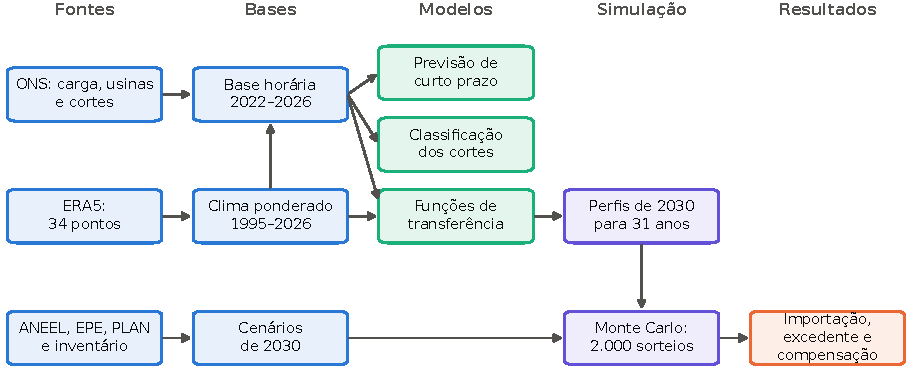
\includegraphics{fig_pipeline}
\caption{Etapas do estudo, das fontes de dados aos resultados.}
\label{fig:pipeline}
\end{figure}

Os cenários e parâmetros ficam em arquivos YAML e CSV separados do código. As versões das bibliotecas estão fixadas, e as sementes aleatórias são \SementeModelos{} para os modelos e \SementeMC{} para a simulação de Monte Carlo. O projeto começou em uma versão de Python e foi transferido para outra (de 3.14 para 3.13), e a simulação de Monte Carlo produziu os mesmos resultados nas duas. Um conjunto de \NTestes{} testes automatizados verifica a conversão de fusos, as unidades, as junções entre bases, o fechamento do balanço e os casos-limite do simulador, como a exigência de que carga adicional nula reproduza o caso sem data centers. As decisões de método estão numeradas e justificadas em um registro com \NDecisoes{} itens.

\subsection{Repositório dos códigos}
\label{sec:repositorio}

% TODO: ao fechar o relatório, incluir o DOI do Zenodo e conferir se o repositório está acessível ao professor.
O código, a configuração, o manifesto e os testes são versionados com Git em \url{https://github.com/MateusMenezes65/estudo-eolica-x-datacenters}. Os arquivos de dados usam Git LFS e podem ser refeitos pelos \textit{scripts} de coleta. Os resultados deste relatório correspondem ao \textit{commit} \texttt{b0ab7fd}.
      % Estratégias de Gestão dos Dados
\section{Caracterização e Preparação dos Dados}
\label{sec:caracterizacao}

\subsection{Harmonização e qualidade}
\label{sec:qualidade}

Todas as séries foram levadas à mesma convenção: o instante $t$ indica o início da hora, no horário de Brasília. A carga verificada, publicada em intervalos de 30~minutos em UTC, foi convertida e agregada pela média, de modo que o valor em MW médios da hora equivale à energia em MWh. Na reanálise, as variáveis instantâneas (temperatura e vento) foram associadas à hora pela média dos seus dois extremos, e a irradiância, que já é uma média horária, foi apenas deslocada.

O subsistema Nordeste do ONS corresponde a oito estados (AL, BA, CE, PB, PE, PI, RN e SE). O clima é amostrado em \NPontosClima{} pontos: as oito capitais, ponderadas pela população, para a carga; 16~polos eólicos e 10~solares, obtidos por \textit{k-means} sobre as coordenadas das usinas do SIGA, com peso proporcional à potência (Figura~\ref{fig:mapa}). As usinas com dados horários somam \NEol{} conjuntos eólicos (\CapEolConj~GW) e \NSol{} solares (\CapSolConj~GW).

\begin{figure}[htb]
\centering
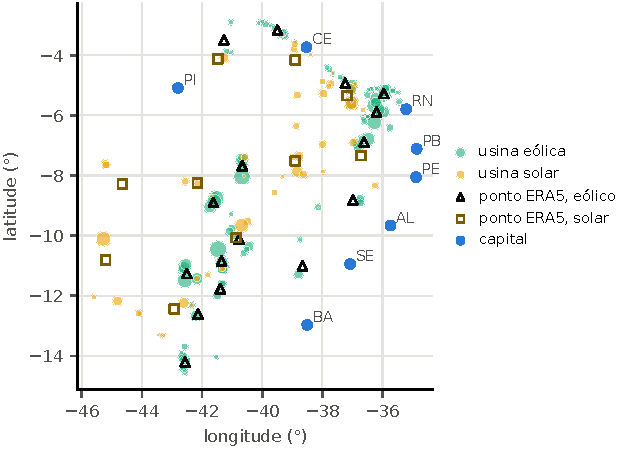
\includegraphics{fig_mapa}
\caption{Usinas eólicas e solares com dados horários no ONS e pontos da reanálise ERA5.}
\label{fig:mapa}
\end{figure}

Não foram encontradas duplicatas nem lacunas internas nas séries centrais, e nenhum valor foi imputado. O balanço do ONS fecha em todas as horas de 2022 a 2025. Entre janeiro e maio de 2026 há \HorasNaoFecha{} horas em que ele não fecha, provavelmente por ainda estar em consistência, e essas horas foram excluídas das comparações com 2026. Três problemas exigiram uma decisão de método e são tratados a seguir: a mudança de definição da carga, o efeito dos cortes sobre a geração e o número reduzido de anos observados.

\subsection{Carga e geração distribuída}
\label{sec:carga}

Em 29/04/2023, o balanço do ONS passou a incluir a micro e minigeração distribuída (MMGD) estimada, tanto na carga quanto na geração solar. Isso produz um degrau de cerca de 0,5~GW na carga (Figura~\ref{fig:carga}) que não corresponde a aumento de consumo. Por isso, a carga modelada vem da série de carga verificada, que informa separadamente a carga global e a MMGD com a mesma definição desde 2022. As duas são modeladas em separado: a forma da carga líquida muda de um ano para outro, à medida que a MMGD reduz o consumo do meio-dia, enquanto a da carga global é mais estável.

\begin{figure}[htb]
\centering
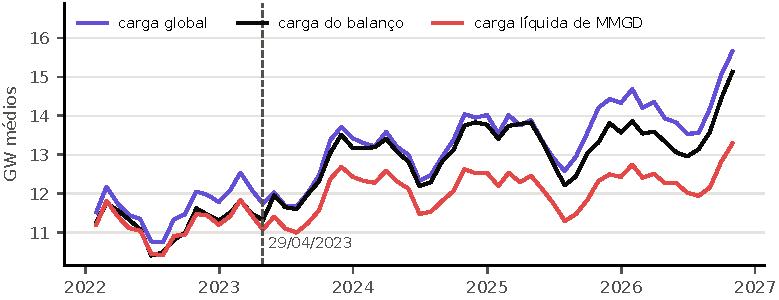
\includegraphics{fig_carga}
\caption{Carga média mensal do Nordeste em três definições.}
\label{fig:carga}
\end{figure}

A carga diária cresce cerca de \CargaGrau\% por grau Celsius (correlação de \CorrTempCarga{} nos dias úteis) e fica \CargaFds\% menor nos fins de semana e feriados. A Figura~\ref{fig:perfis} mostra os perfis por hora e mês. A carga líquida é mínima ao meio-dia e máxima entre 18 e 22~horas. A eólica é mais forte à noite e entre julho e outubro, e a solar só produz de dia. No início da noite, a solar já cessou e a eólica ainda não atingiu o seu máximo.

\begin{figure}[htb]
\centering
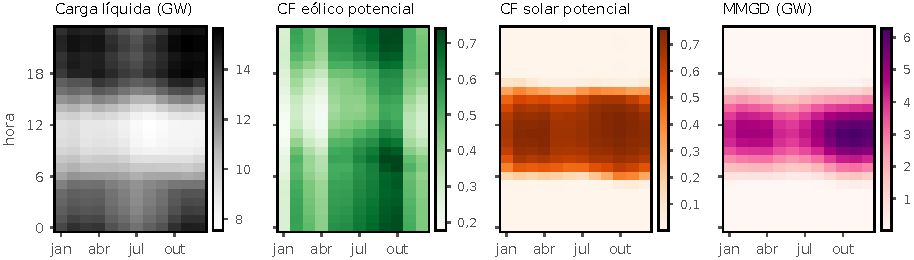
\includegraphics{fig_perfis}
\caption{Perfis médios por hora do dia e mês em 2025.}
\label{fig:perfis}
\end{figure}

\subsection{Geração eólica e cortes}
\label{sec:cortes}

O fator de capacidade (CF) é a razão entre a geração e a capacidade das mesmas usinas na mesma hora. A geração observada, porém, já desconta os cortes, que passaram de \CorteIni\% do potencial em 2022 para \CorteTres\% em 2023, \CorteQuatro\% em 2024 e \CorteCinco\% em 2025 (\CorteTWh~TWh). Com isso, a correlação entre o cubo do vento e o CF observado caiu de \CorrObsIni{} em 2022 para \CorrObsFim{} em 2025 (Figura~\ref{fig:cfvento}).

O alvo adotado é o CF potencial, dado pela soma da geração com a energia cortada apurada pelo ONS, dividida pela capacidade. Com ele, a correlação com o cubo do vento permanece entre \CorrPotMin{} e \CorrPotMax{} em todos os anos. A geração de referência, também publicada pelo ONS, não foi usada como potencial porque fica abaixo da geração verificada em \RefAbaixo\% das horas-usina.

\begin{figure}[htb]
\centering
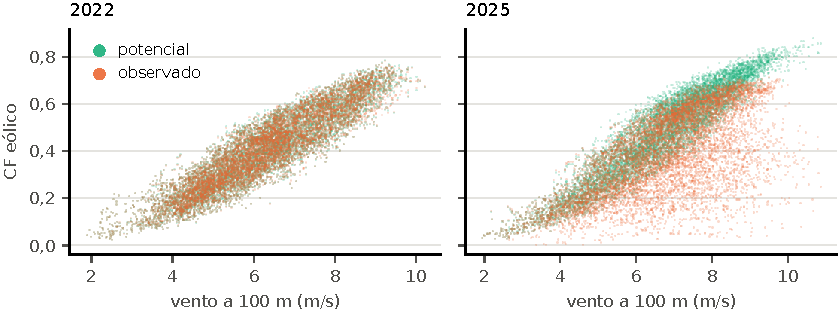
\includegraphics{fig_cf_vento}
\caption{Fator de capacidade eólico observado e potencial em função do vento a 100~m, em 2022 e 2025.}
\label{fig:cfvento}
\end{figure}

\subsection{Anos de clima}
\label{sec:anosclima}

Os quatro anos com dados completos do ONS são, em média, pouco ventosos. Estimado para a frota atual em cada ano da reanálise, o CF eólico varia de \CfMin{} (2009) a \CfMax{} (2012). Entre 31~anos, 2022 é o quarto menos ventoso, 2024 o sétimo, 2023 o décimo primeiro e 2025 o vigésimo terceiro, e a média de 2022 a 2025 é \CfQuatro, contra \CfTrintaUm{} nos 31~anos. Usar somente esses quatro anos levaria a uma estimativa enviesada da geração e não incluiria os anos extremos.
    % Caracterização e Preparação dos Dados
\section{Modelagem e Análise dos Dados}
\label{sec:modelagem}

\subsection{Abordagem}
\label{sec:abordagem}

Prever hora a hora até 2030, usando cada previsão como entrada da seguinte, acumularia erro. Por isso, cada série de 2030 é obtida como o produto de uma forma horária, que depende do clima e do calendário, por um nível anual, definido no cenário. Os termos da Equação~\ref{eq:margem} são
\begin{align}
  G_{\mathrm{NE}}(t) &= H(t) + T(t) + C_e\, f_e(t) + C_s\, f_s(t) + \bar{D}\, f_d(t), \label{eq:geracao}\\
  L_{\mathrm{base}}(t) &= \bar{L}\, f_c(t), \label{eq:carga}
\end{align}
em que $H$ e $T$ são as gerações hidráulica e térmica, $C_e$ e $C_s$ são as capacidades eólica e solar, $f_e$ e $f_s$ são os CFs potenciais, $\bar{D}$ e $\bar{L}$ são os níveis anuais da MMGD e da carga global, e $f_d$ e $f_c$ são as suas formas, com média~1 no ano.

Os modelos usam o \texttt{HistGradientBoosting} do scikit-learn \parencite{pedregosa2011}, que soma árvores de decisão ajustadas sucessivamente aos erros das anteriores. Ele representa relações não lineares, como a curva de potência eólica, e interações, como a de hora com mês, sem que precisem ser especificadas. Os hiperparâmetros são os mesmos em todos os modelos (até 400 árvores, taxa de aprendizado de 0,05, 31 folhas por árvore, no mínimo 40 amostras por folha e regularização L2 igual a 1) e não foram otimizados, para não ajustá-los ao período de teste.

\subsection{Previsão de curto prazo}
\label{sec:curtoprazo}

O primeiro experimento verifica se os modelos capturam as relações entre clima, calendário, carga e geração. Cada hora de 2025 é prevista com 1~hora e 24~horas de antecedência, em 12 dobras mensais, e cada dobra é treinada somente com dados anteriores ao mês testado. As variáveis são o calendário, o clima e os valores do alvo já conhecidos no momento da previsão. Como o clima da hora prevista vem da reanálise, o resultado equivale ao de uma previsão do tempo perfeita e é um limite superior do desempenho em operação.

O modelo supera a melhor referência em pelo menos 10 dos 12 meses em todos os casos (Tabela~\ref{tab:curtoprazo}). O menor ganho é o da solar a 24~horas, em que repetir o valor do dia anterior já tem erro baixo.

\begin{table}[htb]
\centering
\caption{Erro absoluto médio (MAE) da previsão de curto prazo em 2025. A referência é a melhor entre persistência, repetição do dia anterior e repetição da semana anterior.}
\label{tab:curtoprazo}
\footnotesize
\renewcommand{\arraystretch}{1.15}
\begin{tabular}{@{}llrrrr@{}}
\toprule
Alvo & Antecedência & Modelo & Referência & Redução & Meses com erro menor \\
\midrule
\LinhasCurtoPrazo
\bottomrule
\end{tabular}
\end{table}

\subsection{Funções de transferência}
\label{sec:transferencia}

As formas horárias de 2030 vêm de quatro funções de transferência, que recebem clima e calendário e não usam valores passados do alvo (Tabela~\ref{tab:funcoes}). A forma da carga (A0) é a carga global dividida pela média do ano, e a da MMGD (E0) é a razão para a média móvel de 365~dias, o que remove o crescimento da capacidade. As funções eólica (B0) e solar (C0) são treinadas a partir de julho de 2024. No caso da eólica, as usinas mais novas geram de 5\% a 10\% mais com o mesmo vento: um modelo treinado até 2024 e testado em 2025 subestima o CF em \ViesFrota, em média. Na carga e na MMGD, o teste exclui um ano por vez. Na eólica e na solar, o teste usa períodos posteriores ao treino.

\begin{table}[htb]
\centering
\caption{Funções de transferência. O MAE é medido fora do treino, com o do perfil médio por mês e hora entre parênteses (na carga, por mês, dia da semana e hora). A última coluna é a variação do RMSE em relação à versão anterior das variáveis.}
\label{tab:funcoes}
\footnotesize
\renewcommand{\arraystretch}{1.2}
\setlength{\tabcolsep}{4pt}
\begin{tabularx}{\textwidth}{@{}>{\raggedright\arraybackslash}p{2.1cm}>{\raggedright\arraybackslash}X>{\raggedright\arraybackslash}p{2.3cm}>{\raggedright\arraybackslash}p{3.0cm}r@{}}
\toprule
Função & Variáveis & Treino & MAE (perfil médio) & RMSE \\
\midrule
\LinhasFuncoes
\bottomrule
\end{tabularx}
\end{table}

As variáveis foram escolhidas por ablação. Cada variante do modelo é treinada novamente, com ou sem uma variável, e avaliada em anos ou blocos de 12 a 16 meses fora do treino. A diferença de erro tem um intervalo de confiança de 95\% (IC95) calculado por \textit{bootstrap} em blocos de sete dias. Três resultados mudaram a versão anterior dos modelos:
\begin{itemize}
  \item o dia do ano foi retirado das quatro funções. Na eólica e na solar, com apenas 28 meses de treino, o modelo memorizava o tempo de dias específicos, e a retirada reduziu o erro;
  \item o vento de cada um dos 16 polos substituiu o vento médio e o seu cubo. Com a retirada do dia do ano, o RMSE da eólica caiu \GanhoVento\%;
  \item na carga, os graus-hora de resfriamento, a temperatura aparente, a umidade e os feriados menores alteravam o erro em menos de 1\% e saíram, e entrou a média de 24~horas da temperatura.
\end{itemize}

A versão adotada reduz o erro das quatro funções de forma significativa. Como as variáveis foram escolhidas nas mesmas dobras em que o erro é medido, os ganhos são ligeiramente otimistas. Uma variável de ruído, incluída como controle, alterou o erro em até 0,4\%, e diferenças dessa ordem foram desconsideradas.

\begin{figure}[htb]
\centering
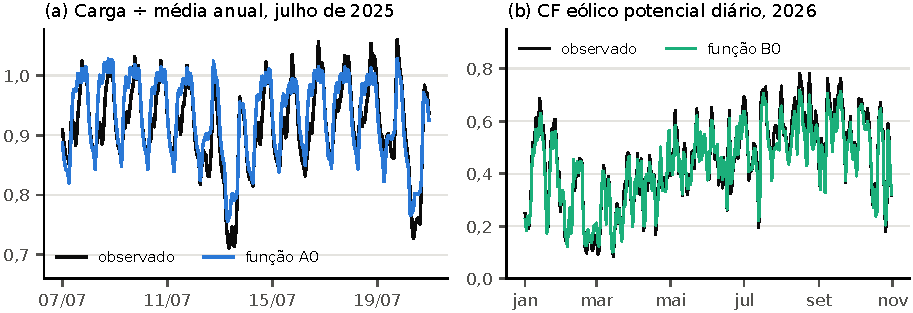
\includegraphics{fig_transferencia}
\caption{Funções de transferência fora do treino: (a) forma da carga em duas semanas de 2025; (b) média diária do CF eólico em 2026.}
\label{fig:transferencia}
\end{figure}

A Figura~\ref{fig:transferencia} compara previsões e observações fora do treino. No CF eólico de 2025, também fora do treino, a correlação horária com o observado é \CorrEol. Nenhuma variável de clima de 1995 a 2021 fica fora da faixa de treino em mais de \Extrap\% das horas, de modo que quase não há extrapolação.

\subsection{Geração hidráulica e térmica}
\label{sec:hidraulica}

A térmica repete a série horária de um dos anos de 2022 a 2025. A hidráulica preserva a energia diária desse mesmo ano, mas a sua distribuição dentro do dia responde à carga líquida, como ocorre no despacho observado (a correlação entre os desvios intradiários das duas é de \CorrHidMin{} a \CorrHidMax{} em 2022--2025):
\begin{equation}
  H(t) = \bar{H}_d + \beta \left[ \ell(t) - \bar{\ell}_d \right],
  \label{eq:hidraulica}
\end{equation}
em que $\bar{H}_d$ é a média do dia, $\ell$ é a carga menos a MMGD e as gerações eólica, solar e térmica, sem cortes, e $\bar{\ell}_d$ é a sua média no dia. O resultado é limitado ao mínimo e ao máximo mensais do ano hidrológico e reajustado para conservar a energia do dia. O coeficiente $\beta$ diminui quando a carga líquida oscila mais: foi de \BetaIni{} em 2022, \BetaVinteCinco{} em 2025 e \BetaCentral{} em 2026. O caso central usa o de 2026, ano observado com a oscilação mais próxima da simulada para 2030.

\subsection{Cenários}
\label{sec:cenarios}

Os cenários combinam quatro níveis de data centers e três de capacidade eólica (Tabela~\ref{tab:cenarios}). A carga sem data centers é a da segunda revisão do PLAN \parencite{plan_2rq} menos a parcela de data centers nela incluída, para que esta não seja contada duas vezes. O cenário alto usa também um inventário de \NProjetosDC{} projetos, levantado em portarias, processos da ANEEL e imprensa setorial. Como a projeção oficial já é expressa em carga na rede, não se aplica o índice de eficiência energética do data center (PUE). O cadastro da ANEEL não informa datas para os projetos fora de operação, e por isso a expansão eólica é definida pela fase dos empreendimentos.

\begin{table}[htb]
\centering
\caption{Níveis adotados para 2030.}
\label{tab:cenarios}
\footnotesize
\renewcommand{\arraystretch}{1.15}
\setlength{\tabcolsep}{4pt}
\begin{tabularx}{\textwidth}{@{}llr>{\raggedright\arraybackslash}X@{}}
\toprule
Dimensão & Cenário & Valor & Definição \\
\midrule
\LinhasCenarios
\bottomrule
\end{tabularx}
\end{table}

\subsection{Simulação de Monte Carlo}
\label{sec:montecarlo}

Cada um dos \NSorteios{} sorteios combina três elementos:
\begin{itemize}
  \item um ano meteorológico entre 1995 e 2025, que define as formas de carga e MMGD e os CFs eólico e solar, dispostos no calendário de 2030;
  \item um ano hidrológico entre 2022 e 2025, que define a energia hidráulica diária e a térmica;
  \item blocos de sete dias de resíduos fora da amostra, das quatro séries em conjunto, tirados de uma janela de 14~dias em torno da mesma época do ano.
\end{itemize}

Os resíduos são necessários porque as funções de transferência estimam médias, com menos variação do que as séries observadas. Eles vêm do período de julho de 2024 a outubro de 2026 e são centrados por mês, para não alterar o nível médio. Com eles, o desvio-padrão horário do CF eólico de 2025, fora da amostra, é \DpSim, contra \DpObs{} observado.

O mesmo sorteio é usado em todos os cenários, o que permite calcular diferenças pareadas. São reportados a média e os percentis 5 e 95 (P5 e P95) dos sorteios. Como estes repetem 31 anos meteorológicos e quatro hidrológicos, aumentar o seu número não reduz a incerteza devida à amostra de anos. Essa incerteza é estimada à parte, por reamostragem dos anos com reposição (4.000 reamostras), e informada como IC95 da média.

A compensação eólica é calculada por dois critérios principais. O primeiro iguala a energia anual dos data centers. O segundo iguala a importação anual à do caso sem data centers, e a capacidade necessária é obtida por bisseção.

\subsection{Classificação dos cortes}
\label{sec:classificador}

Também foi testado um classificador das horas com corte eólico, com variáveis conhecidas antes do evento. Para o corte por razão energética, a área sob a curva precisão-revocação ficou entre \PrMin{} e \PrMax, contra \AcasoMin{} a \AcasoMax{} ao acaso. As probabilidades, porém, não são estáveis: a fração de horas com corte, por qualquer motivo, passou de \HorasCorteIni\% em 2022 para \HorasCorteFim\% em 2025, e o modelo treinado até um ano erra o nível do seguinte. Por isso o classificador não foi aplicado a 2030, e o simulador calcula apenas o excedente.
         % Modelagem e Análise dos Dados
\section{Apresentação e Discussão dos Resultados}
\label{sec:resultados}

\subsection{Verificação do simulador}
\label{sec:verificacao}

Antes de ser aplicado a 2030, o simulador foi comparado com o balanço observado de 2022 a 2026. A importação observada é calculada com os cortes somados à geração, para ter o mesmo conceito da simulada. No primeiro teste, o simulador recebe o clima, a hidrologia e os níveis observados de cada ano, e usa os modelos finais. No segundo, os modelos são treinados sem o ano testado, e os resíduos desse ano também são excluídos (Tabela~\ref{tab:verificacao}).

\begin{table}[H]
\centering
\caption{Importação anual observada e simulada com os níveis observados de cada ano (TWh). Em 2026, janeiro a outubro, nas horas em que o balanço do ONS fecha.}
\label{tab:verificacao}
\footnotesize
\renewcommand{\arraystretch}{1.15}
\begin{tabular}{@{}lrrr@{}}
\toprule
Ano & Observada & Simulada, modelos finais (erro) & Simulada, ano fora do treino (erro) \\
\midrule
\LinhasVerificacao
\bottomrule
\end{tabular}
\end{table}

Com os modelos finais, o erro vai de \ErroRetroMin\% a \ErroRetroMax\%. Fora da amostra, o simulador subestima a importação em todos os anos, de \ErroForaMenor\% a \ErroForaMaior\%, com os maiores erros em 2025 e 2026. Para localizar a origem do erro, as formas simuladas, isto é, a variação de cada série ao longo do ano em torno da sua média, foram trocadas pelas observadas, e a regra hidráulica foi mantida. Com isso, o erro de 2025 cai para menos de 1\%, e o de 2026, para \ErroFormasMin\%. A maior parte do erro desses dois anos vem, portanto, das formas. Nenhuma das séries o explica sozinha. Os desvios de 2025 e 2026 em relação aos modelos diferem dos de outros anos, dos quais vêm os resíduos sorteados, e por isso o sorteio os reproduz apenas em parte.

Para 2026 há um segundo backtest, com os níveis do cenário de 2026 no lugar dos observados (Figura~\ref{fig:backtest}). Com clima e hidrologia sorteados (A), a importação observada de \ObsVinteSeis~TWh fica no percentil \PercVinteSeis{} da distribuição (P5--P95 de \AMin{} a \AMax~TWh). Essa comparação não é uma previsão, pois os modelos finais usam dados até outubro de 2026. Com clima e hidrologia observados e modelos treinados até 2025 (B), o simulador obtém \BVinteSeis~TWh (\ErroBVinteSeis\%). A margem horária simulada tem correlação de \CorrBVinteSeis{} com a observada e o mesmo sinal em \SinalBVinteSeis\% das horas. 

O erro é menor do que o da Tabela~\ref{tab:verificacao} porque, neste teste, as séries simuladas não são ajustadas às médias observadas. A geração eólica simulada fica 3\% abaixo da observada (com os cortes somados), e a carga, 1\% acima da que fecha o balanço do ONS. As duas diferenças aumentam a importação simulada e compensam parte da subestimação.

\begin{figure}[H]
\centering
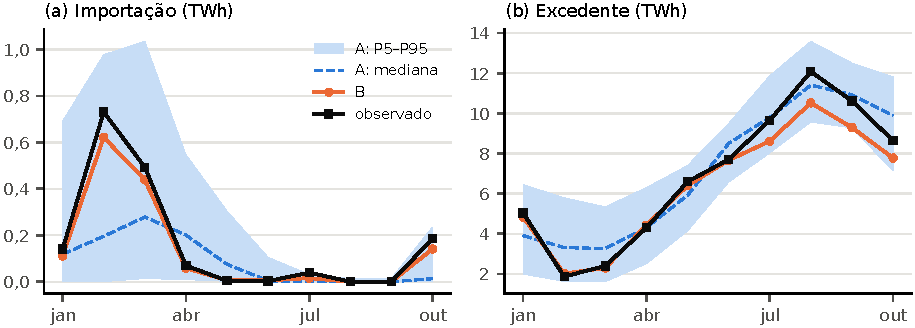
\includegraphics{fig_backtest}
\caption{Importação e excedente mensais de 2026, observados e simulados com os níveis do cenário de 2026. A: clima e hidrologia sorteados. B: clima e hidrologia observados.}
\label{fig:backtest}
\end{figure}

Esses testes indicam que o nível da importação de 2030 tende a estar subestimado. O nível depende também das hipóteses, sobretudo do despacho hidráulico, do nível da carga, da expansão eólica e da data de entrada dos data centers.

\subsection{Importação e excedente em 2030}
\label{sec:importacao2030}

A Tabela~\ref{tab:resultados} resume os resultados. Sem novos data centers e com a expansão eólica base, o Nordeste precisaria importar em média \ImpSem~TWh em 2030, em \HorasSem{} horas do ano. No cenário central, a importação média é de \ImpCen~TWh, em \HorasCen{} horas (\PctHorasCen\% do ano). Um simulador determinístico, que usa os perfis observados de 2022 a 2025 no lugar dos sintéticos, chega a valores próximos: \DetSem~TWh sem data centers e \DetCen~TWh no cenário central. A região continua exportadora em todos os cenários: o excedente médio cai de \ExcSem{} para \ExcCen~TWh no cenário central, e a parcela acima do limite de exportação de 21~GW cai de \ExcLimSem{} para \ExcLimCen~TWh.

\begin{table}[H]
\centering
\caption{Resultados para 2030: média dos sorteios, com P5--P95 entre colchetes. Horas e excedente referem-se à eólica base.}
\label{tab:resultados}
\footnotesize
\renewcommand{\arraystretch}{1.15}
\setlength{\tabcolsep}{5pt}
\begin{tabular}{@{}lrlrrrr@{}}
\toprule
 & & \multicolumn{3}{c}{Importação (TWh)} & & \\
\cmidrule(lr){3-5}
Data centers & MWmed & Eólica base & Eólica baixa & Eólica alta & Horas & Excedente (TWh) \\
\midrule
\LinhasResultados
\bottomrule
\end{tabular}
\end{table}

A importação varia muito de um ano para outro. No cenário central, os percentis 5 e 95 são \ImpCenPCinco{} e \ImpCenPNoventa~TWh, e as distribuições dos cenários se sobrepõem (Figura~\ref{fig:distribuicao}a): a mediana do cenário central (\ImpCenMed~TWh) é menor que o P95 do caso sem data centers (\ImpSemPNoventa~TWh). A maior parte dessa variação vem do clima (Figura~\ref{fig:anos}a). A média do cenário central por ano meteorológico vai de \ImpAnoMin~TWh, com o clima de 2012, a cerca de \ImpAnoMax~TWh, com o de 2009 ou 2020. Na decomposição da variância da importação anual entre os \NSorteios{} sorteios do cenário central, o ano meteorológico responde por \VarClima\%, o ano hidrológico por \VarHidro\% e o restante, que reúne os resíduos e a interação entre os dois anos, por \VarRes\%. O IC95 da média, que considera o número limitado de anos, é de \IcCenMin{} a \IcCenMax~TWh no cenário central e de \IcSemMin{} a \IcSemMax~TWh sem data centers.

\begin{figure}[htb]
\centering
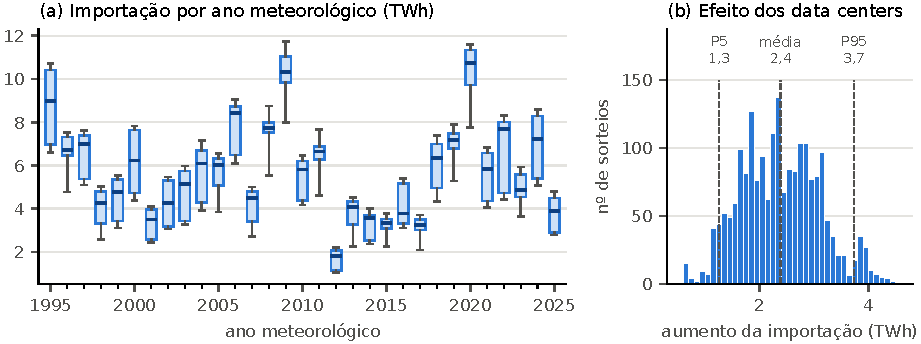
\includegraphics{fig_anos_efeito}
\caption{Cenário central com eólica base: (a) importação anual dos sorteios de cada ano meteorológico, com caixa de P25 a P75, traço na mediana e hastes de P5 a P95; (b) aumento da importação causado pelos data centers em cada um dos \NSorteios{} sorteios, em relação ao caso sem data centers.}
\label{fig:anos}
\end{figure}

\begin{figure}[H]
\centering
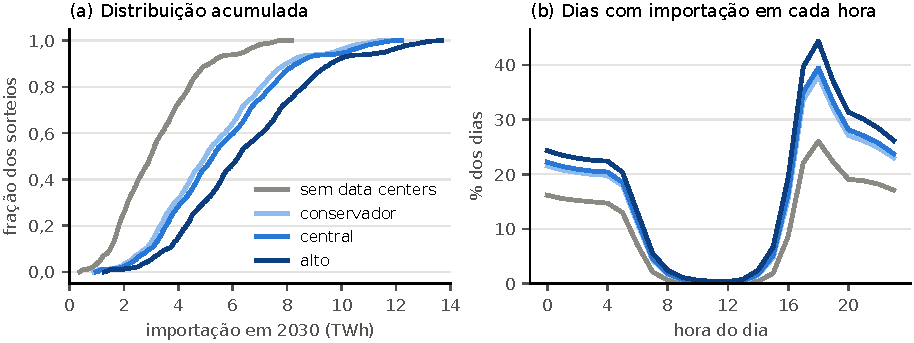
\includegraphics{fig_distribuicao}
\caption{Resultados de 2030 com eólica base: (a) distribuição acumulada da importação anual; (b) percentual de dias com importação em cada hora.}
\label{fig:distribuicao}
\end{figure}

A importação concentra-se no fim da tarde e à noite (Figura~\ref{fig:distribuicao}b). Às 18~horas, quando a solar já cessou e a eólica ainda não subiu, há importação em \PctDezoitoCen\% dos dias no cenário central, contra \PctDezoitoSem\% sem data centers. De madrugada o percentual fica próximo de \PctMadrugada\%, e entre 9 e 13~horas é quase nulo devido ao excedente característico das horas de maior irradiância solar.

\subsection{Efeito dos data centers}
\label{sec:efeito}

Em resumo, no cenário central, os data centers aumentam a importação em \EfCen~TWh por ano (P5--P95 de \EfCenMin{} a \EfCenMax, Figura~\ref{fig:anos}b) e em \EfHoras{} horas. Essa faixa é cerca de três vezes mais estreita que a do nível da importação, porque os dois cenários são comparados no mesmo sorteio, com o mesmo clima. O sinal é positivo por construção, pois a mesma carga adicional é somada a cada sorteio e aumenta a demanda do sistema. No entanto, o que interessa é o aspecto temporal: o aumento de importação equivale a \EfPct\% da energia consumida pelos data centers. Os outros \Absorcao\% são atendidos por geração que, sem eles, seriam horas de excedente. O efeito é de \EfBaixa~TWh com eólica baixa e de \EfAlta~TWh com eólica alta, e o IC95 do valor médio, com eólica base, é de \IcEfMin{} a \IcEfMax~TWh. Não se pode concluir que esse consumo de datacenters evite cortes na mesma proporção em que é atendido pelas horas de excedentes, afinal, parte dos cortes decorre de restrições da rede não representadas. No entanto, o insight importante extraído foi: o papel de aliviar a rede elétrica da sobreoferta de fontes renováveis.

\subsection{Compensação eólica}
\label{sec:compensacao}

Para gerar em um ano a energia consumida pelos data centers do cenário central são necessários \CompEnergia~GW de eólica além da base. Com essa capacidade, a importação média ainda seria de \ImpComEnergia~TWh, acima dos \ImpSem~TWh do caso sem data centers (Figura~\ref{fig:compensacao}). Para voltar a esse nível são necessários \CompImp~GW (P5--P95 de \CompImpMin{} a \CompImpMax), ou \CompRazao{} vezes mais. Para igualar o número de horas com importação, o valor é de \CompHoras~GW. Nos demais cenários, a razão entre os dois primeiros critérios fica entre \RazaoMin{} e \RazaoMax{} e aumenta com a frota eólica.

\begin{figure}[H]
\centering
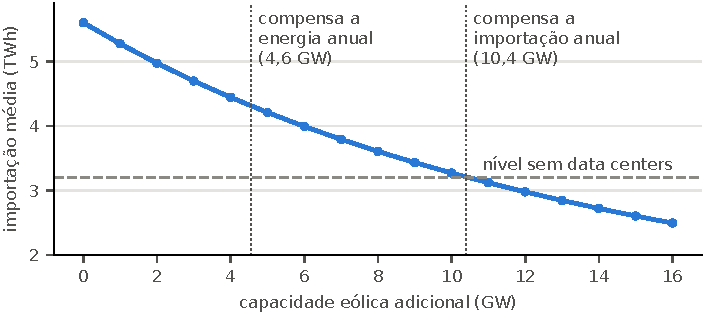
\includegraphics{fig_compensacao}
\caption{Importação média em 2030 no cenário central em função da capacidade eólica adicional (300 sorteios).}
\label{fig:compensacao}
\end{figure}

A diferença conceitual entre essas métricas decorre do perfil da geração. As horas de importação que restam são as de vento fraco, e nelas cada GW adicional gera pouco. Dada a convexidade do gráfico, nota-se que impacto marginal do aumento de geração decresce, pois este é acompanhado de uma redução de horas de importação, para as quais ele contribui no total anual. O cálculo supõe que as novas usinas têm o mesmo perfil horário da frota atual. Uma expansão em locais com regime de vento complementar, ou o armazenamento de energia, mudaria esses valores, mas essas alternativas não foram avaliadas.

\subsection{Sensibilidades}
\label{sec:sensibilidades}

A Figura~\ref{fig:sensibilidades} mostra quanto a importação do cenário central muda quando uma hipótese é alterada. As mais influentes são o despacho hidráulico, o nível da carga, a expansão eólica e a data de entrada dos data centers.

\begin{figure}[H]
\centering
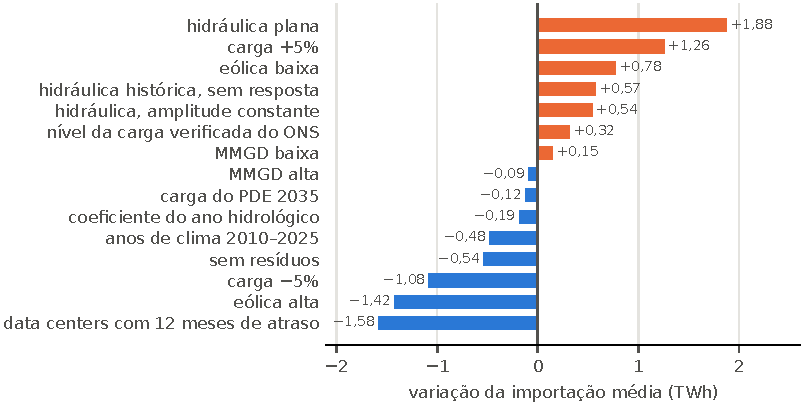
\includegraphics{fig_sensibilidades}
\caption{Variação da importação média do cenário central, com eólica base, em relação à referência (500 sorteios comuns).}
\label{fig:sensibilidades}
\end{figure}

\subsection{Discussão}
\label{sec:discussao}

A variação entre anos encontrada aqui concorda com \textcite{bloomfield2016}, que consideram insuficientes menos de dez anos de dados para o planejamento. A reanálise atende a esse requisito para o vento e a irradiância, mas os quatro anos hidrológicos não. O sorteio também trata o ano meteorológico e o hidrológico como independentes.

\textcite{staffell2016} representam a mudança da frota ao simular cada parque. Aqui, com uma única função para a região, foi preciso treinar em dados recentes, porque as usinas novas geram mais com o mesmo vento. O CF potencial depende da energia cortada apurada pelo ONS, cuja geração de referência mudou ao longo do período, e parte do aumento observado pode vir dessa mudança. A separação entre avaliação \textit{ex ante} e \textit{ex post}, usada por \textcite{hyndman2010}, ajudou a localizar o erro: em 2026, a importação observada é compatível com a distribuição sorteada, e foi o teste com o clima conhecido que revelou a subestimação.

Os picos de importação devem ser lidos com cautela. A média do pico anual é de \PicoSem~GW sem data centers e de \PicoCen~GW no cenário central, acima do maior fluxo de importação registrado de 2022 a 2025 (\FluxoMax~GW). A térmica segue o despacho histórico e não reage à falta de geração, e o estudo não encontrou um limite de importação documentado. Os valores indicam a necessidade calculada se nada mais respondesse e não representam risco de falta de suprimento. Por fim, a projeção oficial de data centers quase triplicou entre a versão original do PLAN e a sua segunda revisão, de modo que os cenários devem ser atualizados a cada nova publicação.
        % Apresentação e Discussão dos Resultados
\section{Conclusões}
\label{sec:conclusoes}

Este trabalho estimou como a entrada de data centers e a expansão eólica mudam o balanço horário do subsistema Nordeste em 2030. Os resultados valem para os cenários adotados e respondem à pergunta da Seção~\ref{sec:problema} da seguinte forma.

Com a projeção oficial vigente (\DcRqDois~MWmed) e a expansão eólica base, os data centers aumentam a necessidade de importação em \EfCen~TWh por ano, de \ImpSem{} para \ImpCen~TWh em média, e em \EfHoras{} horas. O aumento equivale a \EfPct\% da energia que consomem. A região continua exportadora, com excedente médio de \ExcCen~TWh, contra \ExcSem~TWh sem data centers. O aumento da importação concentra-se no fim da tarde e à noite.

Compensar a energia anual dos data centers exige \CompEnergia~GW de eólica adicional. Compensar o aumento da importação exige \CompImp~GW, porque a eólica adicional produz pouco nas horas em que falta geração. Um balanço anual equilibrado não garante, portanto, o atendimento horário.

A importação varia muito com o clima do ano: no cenário central, o intervalo de P5 a P95 vai de \ImpCenPCinco{} a \ImpCenPNoventa~TWh. Usar 31 anos de reanálise, em vez dos quatro anos com dados do ONS, foi necessário para representar essa variação.

Do ponto de vista dos dados, três decisões foram determinantes: usar uma série de carga com definição homogênea, modelar o CF eólico potencial no lugar do observado e escolher as variáveis por ablação fora da amostra. As verificações mostraram também o principal limite do método, que é subestimar a importação fora da amostra, sobretudo em 2025 e 2026. O efeito dos data centers varia menos que o nível entre as hipóteses testadas, de \EfSensMin{} a \EfSensMax~TWh, exceto com atraso na sua entrada.

As demais limitações são a ausência da rede elétrica, a hidráulica representada por uma regra, a térmica fixada no histórico, os quatro anos hidrológicos e a carga constante dos data centers. Os próximos passos são representar o redespacho e os limites de intercâmbio, ampliar a série hidrológica e avaliar o armazenamento e a flexibilidade da carga como alternativas à expansão eólica.
        % Conclusões

\clearpage
\singlespacing
\printbibliography[heading=bibintoc,title={Referências Bibliográficas}]

\end{document}
